\section{DLGN:  Disentangling the computation in DNNs with ReLUs}\label{sec:dlgn}
In this section, we show experimental results comparing performance of standard DNNs with their DGN and DLGN counterparts on CIFAR-10 and CIFAR-100. In what follows, we use the notation DGN$(\xf,\xv)$ and DLGN$(\xf,\xv)$ where $\xf$ and $\xv$ denote the input to the value and feature networks respectively. In this notation, DGN$(x,x)$ will mean that both the value and feature network of the DGN is provided with the image as input, and DLGN$(x,\mathbf{1})$ will mean that the feature network is given with the image as input and the value network is given with $\mathbf{1}$ as input. We consider $3$ DNN architectures, the C4GAP (a $4$ layer convolution network with $128$ filters in each layer followed by global-average-pooling, see \Cref{fig:dgn}) VGG-16 and ResNet-110. %VGG-16 and ResNet-110 are chosen for their state of the art performance on standard datasets namely CIFAR-10 and CIFAR-100. 

\textbf{Result I.} C4GAP chosen as a toy network to experimentally demonstrate the fact that computations in the weight/value network is \emph{disentangled in the path space}, i.e., destroying the layer-by-layer or providing a constant $\mathbf{1}$ input does not destroy the performance as shown in \Cref{tb:permute}.

\textbf{Result II.} 

%Recall that in a DLGN, the gating/feature network is a deep linear network without non-linearities, and hence is disentangled by construction. We claimed in \Cref{sec:intro} that the weight/value network is \emph{disentangled in the path space}, for which, as promised we presented theoretical insights in \Cref{sec:analysis}, and now we will provide the supporting experimental evidence. 



%will experimentally compared DNNs with their DGN and DLGN counterparts, to show how the `disentangled and interpretable' computations in a DLGN recover major part of the performance of DNNs. Recall that the gating/


%This also implies that while non-linearity in ReLU causes entanglement (and hence non-interpretability), the major function of the ReLU as gates is to lift the layer-by-layer computations in the gating/feature network to the path-by-path computations in the weight/value network. 
 

%In this section, we turn to the issues of entanglement and `black box'-ness. We start by noting that the performance in the \emph{learnable gates} setting of the DGN show us that the DGN is not only conceptually similar to the DNN, but also empirically approximate to the DNN. In this paper, we modify the DGN to obtain the LGLN. In particular, the LGLN (\Cref{fig:lgln}) is same as the DGN in which (i) the ReLUs in the feature network are replaced with identity activations, and (ii) the input to the value network is $\mathbf{1}$ (see bottom network of LGLN in \Cref{fig:lgln} and the input to the value network of the DGN in \Cref{fig:dgn}). We now discuss how the LGLN disentangles the computations into two linear structures to show that the commonly held view of sophisticated structures are learnt in a layer-by-layer manner is misconceived.  From now on, as it is with the DGN, we will refer to the top part of the LGLN as its feature network and the bottom part as its value network. 



%Continuing with the `learning in gates + learning in the weights given gates' interpretation, using LGLN (\Cref{fig:lgln}), we disentangle both `learning in the gates' as well as `learning in the weights given gates'. 


%We now elaborate on why these changes are needed in the LGLN and how disentangling is achieved.

%$\bullet$ \textbf{Disentangling Feature Network.}  %The gates themselves encode binary information and are triggered by their pre-activations.In a DGN, the transformation from the input to the pre-activation to the gates happens through the hidden layers, in which the linear and non-linear operations are entangled. The hidden layers are not interpretable, and we have to fall back to sophisticated structures being learnt in the hidden layers as an explanation for why it is possible to learn useful pre-activations (as hence useful gates). In LGLN, the non-linear ReLUs are removed, and the transformation in linear, i.e., while the learning of pre-activations happens in a layer-by-layer manner, the learnt structures are no longer sophisticated and are interpretable in terms of standard linear algebra. We will call this \textbf{primal linearity}. Primal linearity is ensured via construction itself and needs no further theoretical justification, and in what follows, we experimentally verify in \Cref{sec:exp} that linearly learnt pre-activations does not degrade performance significantly, when compared to state of the art.

%$\bullet$ \textbf{Disentangling Value Network.} %Note that the value network of the LGLN and that of the DGN are the same, except that in the DGN the value network is given $x\in\R^{\din}$ as the input and in the LGLN it is a constant $\mathbf{1}\in\R^{\din}$ instead.  We show via experiments in \Cref{sec:exp} that destroying the layer-by-layer structure and the constant $\mathbf{1}$ does not degrade performance. These results are counter intuitive, surprising, and more importantly difficult to reconcile with using the `sophisticated features are learnt in a layer-by-layer' explanation. However, we argue that these surprising results can be readily explained using the NPK expression in \Cref{th:fcprev}.  Note that in a DGN, learning the weights with fixed gates amounts to learning a linear model in the dual variables, i.e., learning $\hat{y}_{\text{DGN}}(x)=\ip{\phi_{\Tf}(x), v_{\Tv}}$. We called this \textbf{dual linearity} and in \Cref{sec:prelim} showed that dual linearity has a kernel interpretation in terms of the NPK in \Cref{th:fcprev}. 
%Thus, giving a constant $\mathbf{1}$ input would mean that $\ip{x,x'}=\din$, and the expression on the right reduces to $d \cdot \sigma^{2(d-1)}\cdot \din\cdot \textbf{overlap}(x,x')$. Now a previously unnoticed fact is that $\textbf{overlap}(x,x')$ is invariant to layer permutations, which implies destroying the layer-by-layer structure does not hurt. In short, the main role of the gating non-linearity is to lift the computations from the primal to the dual space. In the dual space, the right way to interpret the computations is path-by-path and the question of sophisticated structures being learnt in the layers is irrelevant.
%However, in terms of the dual variables, the constant $\mathbf{1}$ has the following interpretation: the neural path value is a vector specifying the contribution of each path to the final output and the neural path feature is a vector specifying the path activity (from \Cref{def:npf-npv} $\phi(x,p)=x\cdot A(x,p)$, and since input is $1$, we have $\phi(x,p)=A(x,p)$), i.e., which path to be selected and which one to be left out in the output. The destruction of layers is possible due to the permutation invariance property of the NPK itself which was unnoticed in prior work. 

%In what follows, in \Cref{th:fc}, we first restate Theorem 5.1 in \cite{npk} (i.e., \Cref{th:fcprev}) so as to explicitly capture the permutation invariance. In order to build a  more complete picture, we extend the dual view to cover the cases of convolution with global pooling and skip connections. We then present the aforementioned experimental results in \Cref{sec:exp}.

%What happens when we give $\mathbf{1}$ input to value network?

%What happens when we give permute the gates?

%Interpreting DLGN$(x,\mathbf{1})$

%Interpreting DSLGN$(x,\mathbf{1})$

%Power of Depth Alone

\begin{figure}[!b]
\centering
\begin{minipage}{0.40\columnwidth}
\centering
\resizebox{0.99\columnwidth}{!}{
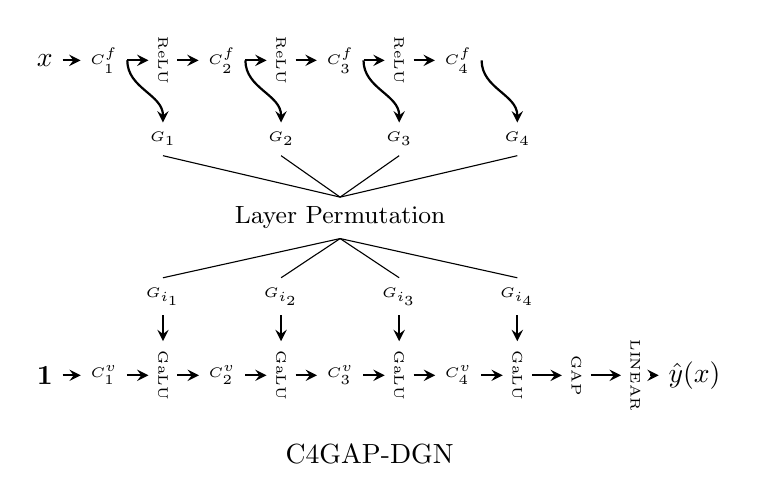
\begin{tikzpicture}
%%%%%%%%%%%%%%%%%%%%%%%%%%%%%%%%%%%%%%%%%%%%%%%%%%%%%%%%%%%%%%%%%
\node []  (fntext)at (4.625,-3.5) {C4GAP-DGN};

%\node []  (output) at (7.5,1.5) {$\hat{y}(x)$};


\node [] (dgn-f-c4) at (5.75,1.5){\tiny{$C^{\text{f}}_4$}};


\node [rotate=-90] (dgn-relu-3) at (5,1.5){\tiny{ReLU}};
\node [] (dgn-f-c3) at (4.25,1.5){\tiny{$C^{\text{f}}_3$}};
\draw [-stealth,thick]   (dgn-f-c3.east) -- (dgn-relu-3.south);
\draw [-stealth,thick]   (dgn-relu-3.north) -- (dgn-f-c4.west);


\node [rotate=-90] (dgn-relu-2) at (3.5,1.5){\tiny{ReLU}};
\node [] (dgn-f-c2) at (2.75,1.5){\tiny{$C^{\text{f}}_2$}};
\draw [-stealth,thick]   (dgn-f-c2.east) -- (dgn-relu-2.south);
\draw [-stealth,thick]   (dgn-relu-2.north) -- (dgn-f-c3.west);


\node [rotate=-90] (dgn-relu-1) at (2,1.5){\tiny{ReLU}};
\node [] (dgn-f-c1) at (1.25,1.5){\tiny{$C^{\text{f}}_1$}};
\draw [-stealth,thick]   (dgn-f-c1.east) -- (dgn-relu-1.south);
\draw [-stealth,thick]   (dgn-relu-1.north) -- (dgn-f-c2.west);



\node [] (dgn-f-input) at (0.5,1.5){$x$};
\draw [-stealth,thick]   (dgn-f-input.east) -- (dgn-f-c1.west);




\node []  (dgn-output) at (8.75,-2.5) {$\hat{y}(x)$};
\node [rotate=-90] (dgn-smax) at (8,-2.5){\tiny{LINEAR}};
\draw [-stealth,thick]   (dgn-smax.north)--(dgn-output.west);

\node [rotate=-90] (dgn-gap) at (7.25,-2.5){\tiny{GAP}};
\draw [-stealth,thick]   (dgn-gap.north)--(dgn-smax.south);



\node [rotate=-90] (dgn-galu-4) at (6.5,-2.5){\tiny{GaLU}};
\draw [-stealth,thick]   (dgn-galu-4.north) -- (dgn-gap.south);

\node [] (dgn-v-c4) at (5.75,-2.5){\tiny{$C^{\text{v}}_4$}};
\draw [-stealth,thick]   (dgn-v-c4.east) -- (dgn-galu-4.south);

\node [rotate=-90] (dgn-galu-3) at (5,-2.5){\tiny{GaLU}};
\node [] (dgn-v-c3) at (4.25,-2.5){\tiny{$C^{\text{v}}_3$}};
\draw [-stealth,thick]   (dgn-v-c3.east) -- (dgn-galu-3.south);
\draw [-stealth,thick]   (dgn-galu-3.north) -- (dgn-v-c4.west);



\node [rotate=-90] (dgn-galu-2) at (3.5,-2.5){\tiny{GaLU}};
\node [] (dgn-v-c2) at (2.75,-2.5){\tiny{$C^{\text{v}}_2$}};
\draw [-stealth,thick]   (dgn-v-c2.east) -- (dgn-galu-2.south);
\draw [-stealth,thick]   (dgn-galu-2.north) -- (dgn-v-c3.west);


\node [rotate=-90] (dgn-galu-1) at (2,-2.5){\tiny{GaLU}};
\node [] (dgn-v-c1) at (1.25,-2.5){\tiny{$C^{\text{v}}_1$}};

\draw [-stealth,thick]   (dgn-v-c1.east) -- (dgn-galu-1.south);
\draw [-stealth,thick]   (dgn-galu-1.north) -- (dgn-v-c2.west);




\node [] (dgn-input) at (0.5,-2.5){$\mathbf{1}$};
\draw [-stealth,thick]   (dgn-input.east) -- (dgn-v-c1.west);


\node[] (dgn-gating-1-up) at (2,0.5){\tiny{$G_{1}$}};
\draw [-stealth,thick]   (dgn-f-c1.east) to[out=-90,in=90] (dgn-gating-1-up.north);


\node[] (dgn-gating-2-up) at (3.5,0.5){\tiny{$G_{2}$}};
\draw [-stealth,thick]   (dgn-f-c2.east) to[out=-90,in=90] (dgn-gating-2-up.north);



\node[] (dgn-gating-3-up) at (5,0.5){\tiny{$G_{3}$}};
\draw [-stealth,thick]   (dgn-f-c3.east) to[out=-90,in=90] (dgn-gating-3-up.north);


\node[] (dgn-gating-4-up) at (6.5,0.5){\tiny{$G_{4}$}};
\draw [-stealth,thick]   (dgn-f-c4.east) to[out=-90,in=90] (dgn-gating-4-up.north);





\node[] (dgn-gating-1) at (2,-1.5){\tiny{$G_{i_1}$}};
\draw [-stealth,thick]   (dgn-gating-1.south) -- (dgn-galu-1.west);


\node[] (dgn-gating-2) at (3.5,-1.5){\tiny{$G_{i_2}$}};
\draw [-stealth,thick]   (dgn-gating-2.south) -- (dgn-galu-2.west);



\node[] (dgn-gating-3) at (5,-1.5){\tiny{$G_{i_3}$}};
\draw [-stealth,thick]   (dgn-gating-3.south) -- (dgn-galu-3.west);


\node[] (dgn-gating-4) at (6.5,-1.5){\tiny{$G_{i_4}$}};
\draw [-stealth,thick]   (dgn-gating-4.south) -- (dgn-galu-4.west);



\node[] (permutation) at (4.25,-0.5){\small{Layer Permutation}};

\draw [-]   (dgn-gating-1-up.south) -- (permutation.north);
\draw [-]   (dgn-gating-4-up.south) -- (permutation.north);
\draw [-]   (dgn-gating-2-up.south) -- (permutation.north);
\draw [-]   (dgn-gating-3-up.south) -- (permutation.north);



\draw [-]  (permutation.south) --  (dgn-gating-1.north)  ;
\draw [-]  (permutation.south) --  (dgn-gating-2.north)  ;
\draw [-]  (permutation.south) --  (dgn-gating-3.north)  ;
\draw [-]  (permutation.south) --  (dgn-gating-4.north)  ;

	
\end{tikzpicture}


}
\end{minipage}
\begin{minipage}{0.40\columnwidth}
\centering
\resizebox{0.99\columnwidth}{!}{
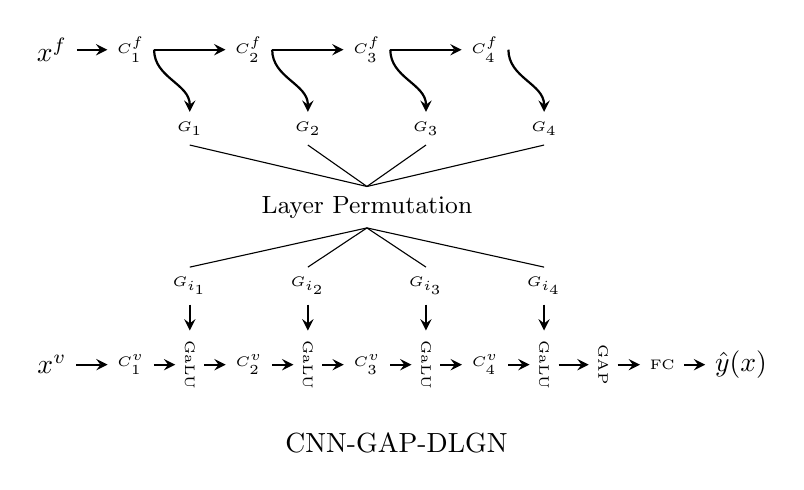
\begin{tikzpicture}
\node []  (fntext)at (-4.625,-3.5) {CNN-GAP-DLGN};

%\node []  (output) at (7.5,1.5) {$\hat{y}(x)$};


\node [] (dgn1-f-c4) at (-3.5,1.5){\tiny{$C^{\text{f}}_4$}};
\node [] (dgn1-f-c3) at (-5,1.5){\tiny{$C^{\text{f}}_3$}};
\node [] (dgn1-f-c2) at (-6.5,1.5){\tiny{$C^{\text{f}}_2$}};
\node [] (dgn1-f-c1) at (-8,1.5){\tiny{$C^{\text{f}}_1$}};
\node [] (dgn1-input-f) at (-9,1.5){$x^{\text{f}}$};
\draw [-stealth,thick]   (dgn1-f-c3.east) -- (dgn1-f-c4.west);
\draw [-stealth,thick]   (dgn1-f-c2.east) -- (dgn1-f-c3.west);
\draw [-stealth,thick]   (dgn1-f-c1.east) -- (dgn1-f-c2.west);
\draw [-stealth,thick]   (dgn1-input-f.east) -- (dgn1-f-c1.west);



\node []  (dgn1-output) at (-0.25,-2.5) {$\hat{y}(x)$};

\node [] (dgn1-smax) at (-1.25,-2.5){\tiny{FC}};
\draw [-stealth,thick]   (dgn1-smax.east)--(dgn1-output.west);

\node [rotate=-90] (dgn1-gap) at (-2,-2.5){\tiny{GAP}};
\draw [-stealth,thick]   (dgn1-gap.north)--(dgn1-smax.west);


\node [rotate=-90] (dgn1-galu-4) at (-2.75,-2.5){\tiny{GaLU}};
\draw [-stealth,thick]   (dgn1-galu-4.north)--(dgn1-gap.south);

\node [] (dgn1-v-c4) at (-3.5,-2.5){\tiny{$C^{\text{v}}_4$}};
\draw [-stealth,thick]   (dgn1-v-c4.east) -- (dgn1-galu-4.south);


\node [rotate=-90] (dgn1-galu-3) at (-4.25,-2.5){\tiny{GaLU}};
\draw [-stealth,thick]   (dgn1-galu-3.north) -- (dgn1-v-c4.west);

\node [] (dgn1-v-c3) at (-5,-2.5){\tiny{$C^{\text{v}}_3$}};
\draw [-stealth,thick]   (dgn1-v-c3.east) -- (dgn1-galu-3.south);


\node [rotate=-90] (dgn1-galu-2) at (-5.75,-2.5){\tiny{GaLU}};
\draw [-stealth,thick]   (dgn1-galu-2.north) -- (dgn1-v-c3.west);

\node [] (dgn1-v-c2) at (-6.5,-2.5){\tiny{$C^{\text{v}}_2$}};
\draw [-stealth,thick]   (dgn1-v-c2.east) -- (dgn1-galu-2.south);


\node [rotate=-90] (dgn1-galu-1) at (-7.25,-2.5){\tiny{GaLU}};
\draw [-stealth,thick]   (dgn1-galu-1.north) -- (dgn1-v-c2.west);


\node [] (dgn1-v-c1) at (-8,-2.5){\tiny{$C^{\text{v}}_1$}};
\draw [-stealth,thick]   (dgn1-v-c1.east) -- (dgn1-galu-1.south);


\node [] (dgn1-v-input) at (-9,-2.5){$x^{\text{v}}$};

\draw [-stealth,thick]   (dgn1-v-input.east) -- (dgn1-v-c1.west);


\node[] (dgn1-gating-4-up) at (-2.75,0.5){\tiny{$G_{4}$}};
\draw [-stealth,thick]   (dgn1-f-c4.east) to[out=-90,in=90] (dgn1-gating-4-up.north);


\node[] (dgn1-gating-3-up) at (-4.25,0.5){\tiny{$G_{3}$}};
\draw [-stealth,thick]   (dgn1-f-c3.east) to[out=-90,in=90] (dgn1-gating-3-up.north);



\node[] (dgn1-gating-2-up) at (-5.75,0.5){\tiny{$G_{2}$}};
\draw [-stealth,thick]   (dgn1-f-c2.east) to[out=-90,in=90] (dgn1-gating-2-up.north);


\node[] (dgn1-gating-1-up) at (-7.25,0.5){\tiny{$G_{1}$}};
\draw [-stealth,thick]   (dgn1-f-c1.east) to[out=-90,in=90] (dgn1-gating-1-up.north);





\node[] (dgn1-gating-4) at (-2.75,-1.5){\tiny{$G_{i_4}$}};
\draw [-stealth,thick]   (dgn1-gating-4.south) -- (dgn1-galu-4.west);


\node[] (dgn1-gating-3) at (-4.25,-1.5){\tiny{$G_{i_3}$}};
\draw [-stealth,thick]   (dgn1-gating-3.south) -- (dgn1-galu-3.west);



\node[] (dgn1-gating-2) at (-5.75,-1.5){\tiny{$G_{i_2}$}};
\draw [-stealth,thick]   (dgn1-gating-2.south) -- (dgn1-galu-2.west);


\node[] (dgn1-gating-1) at (-7.25,-1.5){\tiny{$G_{i_1}$}};
\draw [-stealth,thick]   (dgn1-gating-1.south) -- (dgn1-galu-1.west);



\node[] (permutation1) at (-5,-0.5){\small{Layer Permutation}};

\draw [-]   (dgn1-gating-1-up.south) -- (permutation1.north);
\draw [-]   (dgn1-gating-4-up.south) -- (permutation1.north);
\draw [-]   (dgn1-gating-2-up.south) -- (permutation1.north);
\draw [-]   (dgn1-gating-3-up.south) -- (permutation1.north);



\draw [-]  (permutation1.south) --  (dgn1-gating-1.north)  ;
\draw [-]  (permutation1.south) --  (dgn1-gating-2.north)  ;
\draw [-]  (permutation1.south) --  (dgn1-gating-3.north)  ;
\draw [-]  (permutation1.south) --  (dgn1-gating-4.north)  ;


%%%%%%%%%%%%%%%%%%%%%%%%%%%%%%%%%%%%%%%%%%%%%%%%%%%%%%%%%%%%%%%%%
	
\end{tikzpicture}


}
\end{minipage}
%\begin{minipage}{0.30\columnwidth}
%\centering
%\resizebox{0.99\columnwidth}{!}{
%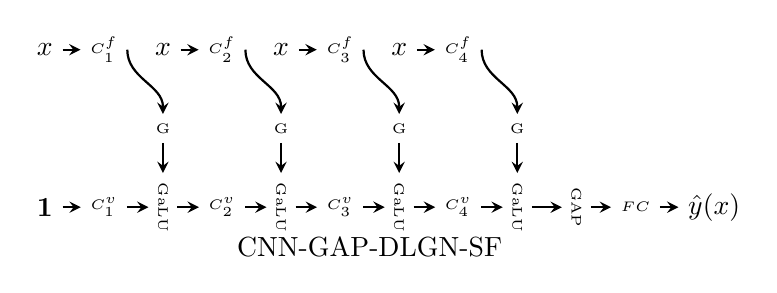
\begin{tikzpicture}
%%%%%%%%%%%%%%%%%%%%%%%%%%%%%%%%%%%%%%%%%%%%%%%%%%%%%%%%%%%%%%%%%
\node []  (fntext)at (4.625,-1) {CNN-GAP-DLGN-SF};

%\node []  (output) at (7.5,1.5) {$\hat{y}(x)$};

\node [] (dgn-f-input) at (0.5,1.5){$x$};
\node [] (dgn-f-c4) at (5.75,1.5){\tiny{$C^{\text{f}}_4$}};

\node [] (dgn-f-x-4) at (5,1.5){$x$};


\node [] (dgn-f-c3) at (4.25,1.5){\tiny{$C^{\text{f}}_3$}};
\node [] (dgn-f-x-3) at (3.5,1.5){$x$};

\node [] (dgn-f-c2) at (2.75,1.5){\tiny{$C^{\text{f}}_2$}};
\node [] (dgn-f-x-2) at (2,1.5){$x$};

\node [] (dgn-f-c1) at (1.25,1.5){\tiny{$C^{\text{f}}_1$}};

\draw [-stealth,thick]   (dgn-f-input.east) -- (dgn-f-c1.west);
\draw [-stealth,thick]   (dgn-f-x-2.east) -- (dgn-f-c2.west);
\draw [-stealth,thick]   (dgn-f-x-3.east) -- (dgn-f-c3.west);
\draw [-stealth,thick]   (dgn-f-x-4.east) -- (dgn-f-c4.west);


\node []  (dgn-output) at (9,-0.5) {$\hat{y}(x)$};



\node [] (dgn-smax) at (8,-0.5){\tiny{$FC$}};
\draw [-stealth,thick]   (dgn-smax.east) -- (dgn-output.west);
;
\node [rotate=-90] (dgn-gap) at (7.25,-0.5){\tiny{GAP}};
\draw [-stealth,thick]   (dgn-gap.north) -- (dgn-smax.west);



\node [rotate=-90] (dgn-galu-4) at (6.5,-0.5){\tiny{GaLU}};

\draw [-stealth,thick]   (dgn-galu-4.north) -- (dgn-gap.south);
\node [] (dgn-v-c4) at (5.75,-0.5){\tiny{$C^{\text{v}}_4$}};
\draw [-stealth,thick]   (dgn-v-c4.east) -- (dgn-galu-4.south);


\node [rotate=-90] (dgn-galu-3) at (5,-0.5){\tiny{GaLU}};
\draw [-stealth,thick]   (dgn-galu-3.north) -- (dgn-v-c4.west);


\node [] (dgn-v-c3) at (4.25,-0.5){\tiny{$C^{\text{v}}_3$}};
\draw [-stealth,thick]   (dgn-v-c3.east) -- (dgn-galu-3.south);


\node [rotate=-90] (dgn-galu-2) at (3.5,-0.5){\tiny{GaLU}};
\draw [-stealth,thick]   (dgn-galu-2.north) -- (dgn-v-c3.west);

\node [] (dgn-v-c2) at (2.75,-0.5){\tiny{$C^{\text{v}}_2$}};
\draw [-stealth,thick]   (dgn-v-c2.east) -- (dgn-galu-2.south);


\node [rotate=-90] (dgn-galu-1) at (2.0,-0.5){\tiny{GaLU}};
\draw [-stealth,thick]   (dgn-galu-1.north) -- (dgn-v-c2.west);

\node [] (dgn-v-c1) at (1.25,-0.5){\tiny{$C^{\text{v}}_1$}};
\draw [-stealth,thick]   (dgn-v-c1.east) -- (dgn-galu-1.south);


\node [] (dgn-v-input) at (0.5,-0.5){$\mathbf{1}$};

\draw [-stealth,thick]   (dgn-v-input.east) -- (dgn-v-c1.west);


\node[] (dgn-gating-1) at (2,0.5){\tiny{G}};
\draw [-stealth,thick]   (dgn-f-c1.east) to[out=-90,in=90] (dgn-gating-1.north);


\node[] (dgn-gating-2) at (3.5,0.5){\tiny{G}};
\draw [-stealth,thick]   (dgn-f-c2.east) to[out=-90,in=90] (dgn-gating-2.north);



\node[] (dgn-gating-3) at (5,0.5){\tiny{G}};
\draw [-stealth,thick]   (dgn-f-c3.east) to[out=-90,in=90] (dgn-gating-3.north);


\node[] (dgn-gating-4) at (6.5,0.5){\tiny{G}};
\draw [-stealth,thick]   (dgn-f-c4.east) to[out=-90,in=90] (dgn-gating-4.north);






\draw [-stealth,thick]   (dgn-gating-1.south) -- (dgn-galu-1.west);



\draw [-stealth,thick]   (dgn-gating-2.south) -- (dgn-galu-2.west);




\draw [-stealth,thick]   (dgn-gating-3.south) -- (dgn-galu-3.west);



\draw [-stealth,thick]   (dgn-gating-4.south) -- (dgn-galu-4.west);





	
\end{tikzpicture}


%}
%\end{minipage}
\caption{$4$ convolutional layers with GAP}
\label{fig:c4gap}
\end{figure}

\begin{comment}
\begin{figure}
\centering
\begin{minipage}{1.0\columnwidth}
\centering
\resizebox{0.99\columnwidth}{!}{
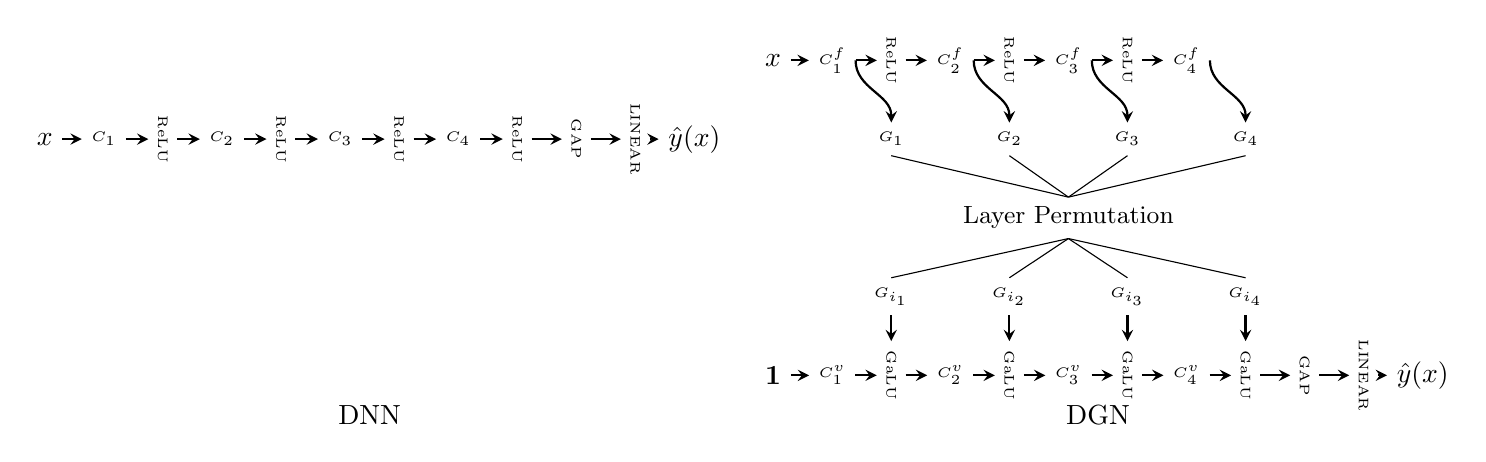
\begin{tikzpicture}
\node []  (dnn-text)at (-4.625,-3) {DNN};

\node []  (dnn-output) at (-0.5,0.5) {$\hat{y}(x)$};
\node [rotate=-90]  (dnn-smax) at (-1.25,0.5) {\tiny{LINEAR}};
\draw [-stealth,thick]   (dnn-smax.north) -- (dnn-output.west);

\node [rotate=-90]  (dnn-gap) at (-2,0.5) {\tiny{GAP}};
\draw [-stealth,thick]   (dnn-gap.north) -- (dnn-smax.south);

\node [rotate=-90] (dnn-relu-4) at (-2.75,0.5){\tiny{ReLU}};
\node [] (dnn-c4) at (-3.5,0.5){\tiny{$C_4$}};
\draw [-stealth,thick]   (dnn-c4.east) -- (dnn-relu-4.south);
\draw [-stealth,thick]   (dnn-relu-4.north) -- (dnn-gap.south);



\node [rotate=-90] (dnn-relu-3) at (-4.25,0.5){\tiny{ReLU}};
\node [] (dnn-c3) at (-5,0.5){\tiny{$C_3$}};
\draw [-stealth,thick]   (dnn-c3.east) -- (dnn-relu-3.south);
\draw [-stealth,thick]   (dnn-relu-3.north) -- (dnn-c4.west);


\node [rotate=-90] (dnn-relu-2) at (-5.75,0.5){\tiny{ReLU}};
\node [] (dnn-c2) at (-6.5,0.5){\tiny{$C_2$}};
\draw [-stealth,thick]   (dnn-c2.east) -- (dnn-relu-2.south);
\draw [-stealth,thick]   (dnn-relu-2.north) -- (dnn-c3.west);

\node [rotate=-90] (dnn-relu-1) at (-7.25,0.5){\tiny{ReLU}};
\node [] (dnn-c1) at (-8,0.5){\tiny{$C_1$}};
\draw [-stealth,thick]   (dnn-c1.east) -- (dnn-relu-1.south);
\draw [-stealth,thick]   (dnn-relu-1.north) -- (dnn-c2.west);



\node [] (dnn-input) at (-8.75,0.5){$x$};
\draw [-stealth,thick]   (dnn-input.east) -- (dnn-c1.west);


%%%%%%%%%%%%%%%%%%%%%%%%%%%%%%%%%%%%%%%%%%%%%%%%%%%%%%%%%%%%%%%%%
\node []  (fntext)at (4.625,-3) {DGN};

%\node []  (output) at (7.5,1.5) {$\hat{y}(x)$};


\node [] (dgn-f-c4) at (5.75,1.5){\tiny{$C^{\text{f}}_4$}};


\node [rotate=-90] (dgn-relu-3) at (5,1.5){\tiny{ReLU}};
\node [] (dgn-f-c3) at (4.25,1.5){\tiny{$C^{\text{f}}_3$}};
\draw [-stealth,thick]   (dgn-f-c3.east) -- (dgn-relu-3.south);
\draw [-stealth,thick]   (dgn-relu-3.north) -- (dgn-f-c4.west);


\node [rotate=-90] (dgn-relu-2) at (3.5,1.5){\tiny{ReLU}};
\node [] (dgn-f-c2) at (2.75,1.5){\tiny{$C^{\text{f}}_2$}};
\draw [-stealth,thick]   (dgn-f-c2.east) -- (dgn-relu-2.south);
\draw [-stealth,thick]   (dgn-relu-2.north) -- (dgn-f-c3.west);


\node [rotate=-90] (dgn-relu-1) at (2,1.5){\tiny{ReLU}};
\node [] (dgn-f-c1) at (1.25,1.5){\tiny{$C^{\text{f}}_1$}};
\draw [-stealth,thick]   (dgn-f-c1.east) -- (dgn-relu-1.south);
\draw [-stealth,thick]   (dgn-relu-1.north) -- (dgn-f-c2.west);



\node [] (dgn-f-input) at (0.5,1.5){$x$};
\draw [-stealth,thick]   (dgn-f-input.east) -- (dgn-f-c1.west);




\node []  (dgn-output) at (8.75,-2.5) {$\hat{y}(x)$};
\node [rotate=-90] (dgn-smax) at (8,-2.5){\tiny{LINEAR}};
\draw [-stealth,thick]   (dgn-smax.north)--(dgn-output.west);

\node [rotate=-90] (dgn-gap) at (7.25,-2.5){\tiny{GAP}};
\draw [-stealth,thick]   (dgn-gap.north)--(dgn-smax.south);



\node [rotate=-90] (dgn-galu-4) at (6.5,-2.5){\tiny{GaLU}};
\draw [-stealth,thick]   (dgn-galu-4.north) -- (dgn-gap.south);

\node [] (dgn-v-c4) at (5.75,-2.5){\tiny{$C^{\text{v}}_4$}};
\draw [-stealth,thick]   (dgn-v-c4.east) -- (dgn-galu-4.south);

\node [rotate=-90] (dgn-galu-3) at (5,-2.5){\tiny{GaLU}};
\node [] (dgn-v-c3) at (4.25,-2.5){\tiny{$C^{\text{v}}_3$}};
\draw [-stealth,thick]   (dgn-v-c3.east) -- (dgn-galu-3.south);
\draw [-stealth,thick]   (dgn-galu-3.north) -- (dgn-v-c4.west);



\node [rotate=-90] (dgn-galu-2) at (3.5,-2.5){\tiny{GaLU}};
\node [] (dgn-v-c2) at (2.75,-2.5){\tiny{$C^{\text{v}}_2$}};
\draw [-stealth,thick]   (dgn-v-c2.east) -- (dgn-galu-2.south);
\draw [-stealth,thick]   (dgn-galu-2.north) -- (dgn-v-c3.west);


\node [rotate=-90] (dgn-galu-1) at (2,-2.5){\tiny{GaLU}};
\node [] (dgn-v-c1) at (1.25,-2.5){\tiny{$C^{\text{v}}_1$}};

\draw [-stealth,thick]   (dgn-v-c1.east) -- (dgn-galu-1.south);
\draw [-stealth,thick]   (dgn-galu-1.north) -- (dgn-v-c2.west);




\node [] (dgn-input) at (0.5,-2.5){$\mathbf{1}$};
\draw [-stealth,thick]   (dgn-input.east) -- (dgn-v-c1.west);


\node[] (dgn-gating-1-up) at (2,0.5){\tiny{$G_{1}$}};
\draw [-stealth,thick]   (dgn-f-c1.east) to[out=-90,in=90] (dgn-gating-1-up.north);


\node[] (dgn-gating-2-up) at (3.5,0.5){\tiny{$G_{2}$}};
\draw [-stealth,thick]   (dgn-f-c2.east) to[out=-90,in=90] (dgn-gating-2-up.north);



\node[] (dgn-gating-3-up) at (5,0.5){\tiny{$G_{3}$}};
\draw [-stealth,thick]   (dgn-f-c3.east) to[out=-90,in=90] (dgn-gating-3-up.north);


\node[] (dgn-gating-4-up) at (6.5,0.5){\tiny{$G_{4}$}};
\draw [-stealth,thick]   (dgn-f-c4.east) to[out=-90,in=90] (dgn-gating-4-up.north);





\node[] (dgn-gating-1) at (2,-1.5){\tiny{$G_{i_1}$}};
\draw [-stealth,thick]   (dgn-gating-1.south) -- (dgn-galu-1.west);


\node[] (dgn-gating-2) at (3.5,-1.5){\tiny{$G_{i_2}$}};
\draw [-stealth,thick]   (dgn-gating-2.south) -- (dgn-galu-2.west);



\node[] (dgn-gating-3) at (5,-1.5){\tiny{$G_{i_3}$}};
\draw [-stealth,thick]   (dgn-gating-3.south) -- (dgn-galu-3.west);


\node[] (dgn-gating-4) at (6.5,-1.5){\tiny{$G_{i_4}$}};
\draw [-stealth,thick]   (dgn-gating-4.south) -- (dgn-galu-4.west);



\node[] (permutation) at (4.25,-0.5){\small{Layer Permutation}};

\draw [-]   (dgn-gating-1-up.south) -- (permutation.north);
\draw [-]   (dgn-gating-4-up.south) -- (permutation.north);
\draw [-]   (dgn-gating-2-up.south) -- (permutation.north);
\draw [-]   (dgn-gating-3-up.south) -- (permutation.north);



\draw [-]  (permutation.south) --  (dgn-gating-1.north)  ;
\draw [-]  (permutation.south) --  (dgn-gating-2.north)  ;
\draw [-]  (permutation.south) --  (dgn-gating-3.north)  ;
\draw [-]  (permutation.south) --  (dgn-gating-4.north)  ;

	
\end{tikzpicture}


}
\resizebox{0.99\columnwidth}{!}{
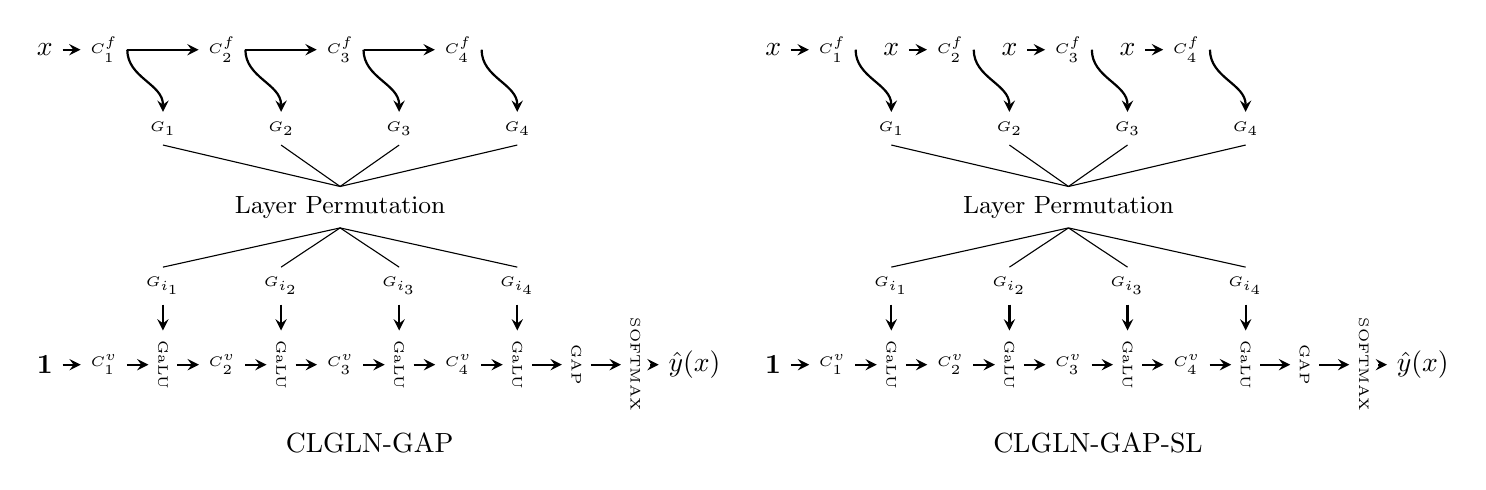
\begin{tikzpicture}
\node []  (fntext)at (-4.625,-3.5) {CLGLN-GAP};

%\node []  (output) at (7.5,1.5) {$\hat{y}(x)$};


\node [] (dgn1-f-c4) at (-3.5,1.5){\tiny{$C^{\text{f}}_4$}};
\node [] (dgn1-f-c3) at (-5,1.5){\tiny{$C^{\text{f}}_3$}};
\node [] (dgn1-f-c2) at (-6.5,1.5){\tiny{$C^{\text{f}}_2$}};
\node [] (dgn1-f-c1) at (-8,1.5){\tiny{$C^{\text{f}}_1$}};
\node [] (dgn1-input-f) at (-8.75,1.5){$x$};
\draw [-stealth,thick]   (dgn1-f-c3.east) -- (dgn1-f-c4.west);
\draw [-stealth,thick]   (dgn1-f-c2.east) -- (dgn1-f-c3.west);
\draw [-stealth,thick]   (dgn1-f-c1.east) -- (dgn1-f-c2.west);
\draw [-stealth,thick]   (dgn1-input-f.east) -- (dgn1-f-c1.west);



\node []  (dgn1-output) at (-0.5,-2.5) {$\hat{y}(x)$};

\node [rotate=-90] (dgn1-smax) at (-1.25,-2.5){\tiny{SOFTMAX}};
\draw [-stealth,thick]   (dgn1-smax.north)--(dgn1-output.west);

\node [rotate=-90] (dgn1-gap) at (-2,-2.5){\tiny{GAP}};
\draw [-stealth,thick]   (dgn1-gap.north)--(dgn1-smax.south);


\node [rotate=-90] (dgn1-galu-4) at (-2.75,-2.5){\tiny{GaLU}};
\draw [-stealth,thick]   (dgn1-galu-4.north)--(dgn1-gap.south);

\node [] (dgn1-v-c4) at (-3.5,-2.5){\tiny{$C^{\text{v}}_4$}};
\draw [-stealth,thick]   (dgn1-v-c4.east) -- (dgn1-galu-4.south);


\node [rotate=-90] (dgn1-galu-3) at (-4.25,-2.5){\tiny{GaLU}};
\draw [-stealth,thick]   (dgn1-galu-3.north) -- (dgn1-v-c4.west);

\node [] (dgn1-v-c3) at (-5,-2.5){\tiny{$C^{\text{v}}_3$}};
\draw [-stealth,thick]   (dgn1-v-c3.east) -- (dgn1-galu-3.south);


\node [rotate=-90] (dgn1-galu-2) at (-5.75,-2.5){\tiny{GaLU}};
\draw [-stealth,thick]   (dgn1-galu-2.north) -- (dgn1-v-c3.west);

\node [] (dgn1-v-c2) at (-6.5,-2.5){\tiny{$C^{\text{v}}_2$}};
\draw [-stealth,thick]   (dgn1-v-c2.east) -- (dgn1-galu-2.south);


\node [rotate=-90] (dgn1-galu-1) at (-7.25,-2.5){\tiny{GaLU}};
\draw [-stealth,thick]   (dgn1-galu-1.north) -- (dgn1-v-c2.west);


\node [] (dgn1-v-c1) at (-8,-2.5){\tiny{$C^{\text{v}}_1$}};
\draw [-stealth,thick]   (dgn1-v-c1.east) -- (dgn1-galu-1.south);


\node [] (dgn1-v-input) at (-8.75,-2.5){$\mathbf{1}$};

\draw [-stealth,thick]   (dgn1-v-input.east) -- (dgn1-v-c1.west);


\node[] (dgn1-gating-4-up) at (-2.75,0.5){\tiny{$G_{4}$}};
\draw [-stealth,thick]   (dgn1-f-c4.east) to[out=-90,in=90] (dgn1-gating-4-up.north);


\node[] (dgn1-gating-3-up) at (-4.25,0.5){\tiny{$G_{3}$}};
\draw [-stealth,thick]   (dgn1-f-c3.east) to[out=-90,in=90] (dgn1-gating-3-up.north);



\node[] (dgn1-gating-2-up) at (-5.75,0.5){\tiny{$G_{2}$}};
\draw [-stealth,thick]   (dgn1-f-c2.east) to[out=-90,in=90] (dgn1-gating-2-up.north);


\node[] (dgn1-gating-1-up) at (-7.25,0.5){\tiny{$G_{1}$}};
\draw [-stealth,thick]   (dgn1-f-c1.east) to[out=-90,in=90] (dgn1-gating-1-up.north);





\node[] (dgn1-gating-4) at (-2.75,-1.5){\tiny{$G_{i_4}$}};
\draw [-stealth,thick]   (dgn1-gating-4.south) -- (dgn1-galu-4.west);


\node[] (dgn1-gating-3) at (-4.25,-1.5){\tiny{$G_{i_3}$}};
\draw [-stealth,thick]   (dgn1-gating-3.south) -- (dgn1-galu-3.west);



\node[] (dgn1-gating-2) at (-5.75,-1.5){\tiny{$G_{i_2}$}};
\draw [-stealth,thick]   (dgn1-gating-2.south) -- (dgn1-galu-2.west);


\node[] (dgn1-gating-1) at (-7.25,-1.5){\tiny{$G_{i_1}$}};
\draw [-stealth,thick]   (dgn1-gating-1.south) -- (dgn1-galu-1.west);



\node[] (permutation1) at (-5,-0.5){\small{Layer Permutation}};

\draw [-]   (dgn1-gating-1-up.south) -- (permutation1.north);
\draw [-]   (dgn1-gating-4-up.south) -- (permutation1.north);
\draw [-]   (dgn1-gating-2-up.south) -- (permutation1.north);
\draw [-]   (dgn1-gating-3-up.south) -- (permutation1.north);



\draw [-]  (permutation1.south) --  (dgn1-gating-1.north)  ;
\draw [-]  (permutation1.south) --  (dgn1-gating-2.north)  ;
\draw [-]  (permutation1.south) --  (dgn1-gating-3.north)  ;
\draw [-]  (permutation1.south) --  (dgn1-gating-4.north)  ;


%%%%%%%%%%%%%%%%%%%%%%%%%%%%%%%%%%%%%%%%%%%%%%%%%%%%%%%%%%%%%%%%%
\node []  (fntext)at (4.625,-3.5) {CLGLN-GAP-SL};

%\node []  (output) at (7.5,1.5) {$\hat{y}(x)$};

\node [] (dgn-f-input) at (0.5,1.5){$x$};
\node [] (dgn-f-c4) at (5.75,1.5){\tiny{$C^{\text{f}}_4$}};

\node [] (dgn-f-x-4) at (5,1.5){$x$};


\node [] (dgn-f-c3) at (4.25,1.5){\tiny{$C^{\text{f}}_3$}};
\node [] (dgn-f-x-3) at (3.5,1.5){$x$};

\node [] (dgn-f-c2) at (2.75,1.5){\tiny{$C^{\text{f}}_2$}};
\node [] (dgn-f-x-2) at (2,1.5){$x$};

\node [] (dgn-f-c1) at (1.25,1.5){\tiny{$C^{\text{f}}_1$}};

\draw [-stealth,thick]   (dgn-f-input.east) -- (dgn-f-c1.west);
\draw [-stealth,thick]   (dgn-f-x-2.east) -- (dgn-f-c2.west);
\draw [-stealth,thick]   (dgn-f-x-3.east) -- (dgn-f-c3.west);
\draw [-stealth,thick]   (dgn-f-x-4.east) -- (dgn-f-c4.west);


\node []  (dgn-output) at (8.75,-2.5) {$\hat{y}(x)$};



\node [rotate=-90] (dgn-smax) at (8,-2.5){\tiny{SOFTMAX}};
\draw [-stealth,thick]   (dgn-smax.north) -- (dgn-output.west);
;
\node [rotate=-90] (dgn-gap) at (7.25,-2.5){\tiny{GAP}};
\draw [-stealth,thick]   (dgn-gap.north) -- (dgn-smax.south);



\node [rotate=-90] (dgn-galu-4) at (6.5,-2.5){\tiny{GaLU}};

\draw [-stealth,thick]   (dgn-galu-4.north) -- (dgn-gap.south);
\node [] (dgn-v-c4) at (5.75,-2.5){\tiny{$C^{\text{v}}_4$}};
\draw [-stealth,thick]   (dgn-v-c4.east) -- (dgn-galu-4.south);


\node [rotate=-90] (dgn-galu-3) at (5,-2.5){\tiny{GaLU}};
\draw [-stealth,thick]   (dgn-galu-3.north) -- (dgn-v-c4.west);


\node [] (dgn-v-c3) at (4.25,-2.5){\tiny{$C^{\text{v}}_3$}};
\draw [-stealth,thick]   (dgn-v-c3.east) -- (dgn-galu-3.south);


\node [rotate=-90] (dgn-galu-2) at (3.5,-2.5){\tiny{GaLU}};
\draw [-stealth,thick]   (dgn-galu-2.north) -- (dgn-v-c3.west);

\node [] (dgn-v-c2) at (2.75,-2.5){\tiny{$C^{\text{v}}_2$}};
\draw [-stealth,thick]   (dgn-v-c2.east) -- (dgn-galu-2.south);


\node [rotate=-90] (dgn-galu-1) at (2.0,-2.5){\tiny{GaLU}};
\draw [-stealth,thick]   (dgn-galu-1.north) -- (dgn-v-c2.west);

\node [] (dgn-v-c1) at (1.25,-2.5){\tiny{$C^{\text{v}}_1$}};
\draw [-stealth,thick]   (dgn-v-c1.east) -- (dgn-galu-1.south);


\node [] (dgn-v-input) at (0.5,-2.5){$\mathbf{1}$};

\draw [-stealth,thick]   (dgn-v-input.east) -- (dgn-v-c1.west);


\node[] (dgn-gating-1-up) at (2,0.5){\tiny{$G_{1}$}};
\draw [-stealth,thick]   (dgn-f-c1.east) to[out=-90,in=90] (dgn-gating-1-up.north);


\node[] (dgn-gating-2-up) at (3.5,0.5){\tiny{$G_{2}$}};
\draw [-stealth,thick]   (dgn-f-c2.east) to[out=-90,in=90] (dgn-gating-2-up.north);



\node[] (dgn-gating-3-up) at (5,0.5){\tiny{$G_{3}$}};
\draw [-stealth,thick]   (dgn-f-c3.east) to[out=-90,in=90] (dgn-gating-3-up.north);


\node[] (dgn-gating-4-up) at (6.5,0.5){\tiny{$G_{4}$}};
\draw [-stealth,thick]   (dgn-f-c4.east) to[out=-90,in=90] (dgn-gating-4-up.north);





\node[] (dgn-gating-1) at (2,-1.5){\tiny{$G_{i_1}$}};
\draw [-stealth,thick]   (dgn-gating-1.south) -- (dgn-galu-1.west);


\node[] (dgn-gating-2) at (3.5,-1.5){\tiny{$G_{i_2}$}};
\draw [-stealth,thick]   (dgn-gating-2.south) -- (dgn-galu-2.west);



\node[] (dgn-gating-3) at (5,-1.5){\tiny{$G_{i_3}$}};
\draw [-stealth,thick]   (dgn-gating-3.south) -- (dgn-galu-3.west);


\node[] (dgn-gating-4) at (6.5,-1.5){\tiny{$G_{i_4}$}};
\draw [-stealth,thick]   (dgn-gating-4.south) -- (dgn-galu-4.west);



\node[] (permutation) at (4.25,-0.5){\small{Layer Permutation}};

\draw [-]   (dgn-gating-1-up.south) -- (permutation.north);
\draw [-]   (dgn-gating-4-up.south) -- (permutation.north);
\draw [-]   (dgn-gating-2-up.south) -- (permutation.north);
\draw [-]   (dgn-gating-3-up.south) -- (permutation.north);



\draw [-]  (permutation.south) --  (dgn-gating-1.north)  ;
\draw [-]  (permutation.south) --  (dgn-gating-2.north)  ;
\draw [-]  (permutation.south) --  (dgn-gating-3.north)  ;
\draw [-]  (permutation.south) --  (dgn-gating-4.north)  ;



	
\end{tikzpicture}


}
\end{minipage}
\caption{$4$ convolutional layers with GAP}
\label{fig:c4gap}
\end{figure}




\begin{figure}[!t]
\centering
\begin{minipage}{1.0\columnwidth}
\centering
\begin{minipage}{0.49\columnwidth}
\resizebox{0.99\columnwidth}{!}{
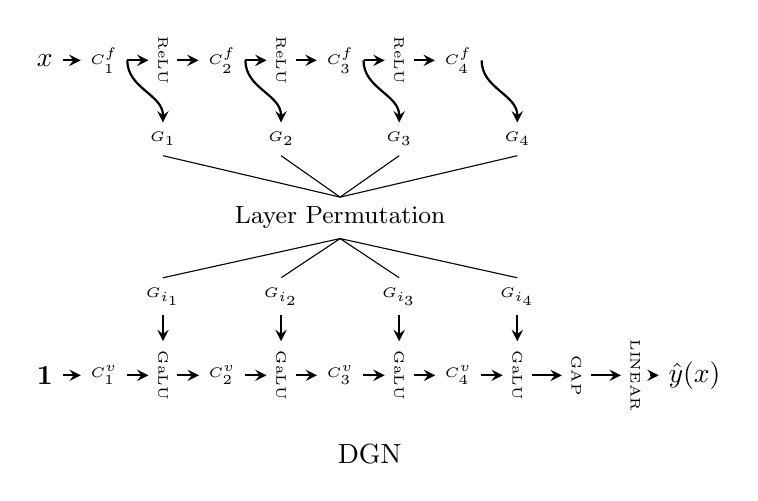
\begin{tikzpicture}
%%%%%%%%%%%%%%%%%%%%%%%%%%%%%%%%%%%%%%%%%%%%%%%%%%%%%%%%%%%%%%%%%
\node []  (fntext)at (4.625,-3.5) {DGN};

%\node []  (output) at (7.5,1.5) {$\hat{y}(x)$};


\node [] (dgn-f-c4) at (5.75,1.5){\tiny{$C^{\text{f}}_4$}};


\node [rotate=-90] (dgn-relu-3) at (5,1.5){\tiny{ReLU}};
\node [] (dgn-f-c3) at (4.25,1.5){\tiny{$C^{\text{f}}_3$}};
\draw [-stealth,thick]   (dgn-f-c3.east) -- (dgn-relu-3.south);
\draw [-stealth,thick]   (dgn-relu-3.north) -- (dgn-f-c4.west);


\node [rotate=-90] (dgn-relu-2) at (3.5,1.5){\tiny{ReLU}};
\node [] (dgn-f-c2) at (2.75,1.5){\tiny{$C^{\text{f}}_2$}};
\draw [-stealth,thick]   (dgn-f-c2.east) -- (dgn-relu-2.south);
\draw [-stealth,thick]   (dgn-relu-2.north) -- (dgn-f-c3.west);


\node [rotate=-90] (dgn-relu-1) at (2,1.5){\tiny{ReLU}};
\node [] (dgn-f-c1) at (1.25,1.5){\tiny{$C^{\text{f}}_1$}};
\draw [-stealth,thick]   (dgn-f-c1.east) -- (dgn-relu-1.south);
\draw [-stealth,thick]   (dgn-relu-1.north) -- (dgn-f-c2.west);



\node [] (dgn-f-input) at (0.5,1.5){$x$};
\draw [-stealth,thick]   (dgn-f-input.east) -- (dgn-f-c1.west);




\node []  (dgn-output) at (8.75,-2.5) {$\hat{y}(x)$};
\node [rotate=-90] (dgn-smax) at (8,-2.5){\tiny{LINEAR}};
\draw [-stealth,thick]   (dgn-smax.north)--(dgn-output.west);

\node [rotate=-90] (dgn-gap) at (7.25,-2.5){\tiny{GAP}};
\draw [-stealth,thick]   (dgn-gap.north)--(dgn-smax.south);



\node [rotate=-90] (dgn-galu-4) at (6.5,-2.5){\tiny{GaLU}};
\draw [-stealth,thick]   (dgn-galu-4.north) -- (dgn-gap.south);

\node [] (dgn-v-c4) at (5.75,-2.5){\tiny{$C^{\text{v}}_4$}};
\draw [-stealth,thick]   (dgn-v-c4.east) -- (dgn-galu-4.south);

\node [rotate=-90] (dgn-galu-3) at (5,-2.5){\tiny{GaLU}};
\node [] (dgn-v-c3) at (4.25,-2.5){\tiny{$C^{\text{v}}_3$}};
\draw [-stealth,thick]   (dgn-v-c3.east) -- (dgn-galu-3.south);
\draw [-stealth,thick]   (dgn-galu-3.north) -- (dgn-v-c4.west);



\node [rotate=-90] (dgn-galu-2) at (3.5,-2.5){\tiny{GaLU}};
\node [] (dgn-v-c2) at (2.75,-2.5){\tiny{$C^{\text{v}}_2$}};
\draw [-stealth,thick]   (dgn-v-c2.east) -- (dgn-galu-2.south);
\draw [-stealth,thick]   (dgn-galu-2.north) -- (dgn-v-c3.west);


\node [rotate=-90] (dgn-galu-1) at (2,-2.5){\tiny{GaLU}};
\node [] (dgn-v-c1) at (1.25,-2.5){\tiny{$C^{\text{v}}_1$}};

\draw [-stealth,thick]   (dgn-v-c1.east) -- (dgn-galu-1.south);
\draw [-stealth,thick]   (dgn-galu-1.north) -- (dgn-v-c2.west);




\node [] (dgn-input) at (0.5,-2.5){$\mathbf{1}$};
\draw [-stealth,thick]   (dgn-input.east) -- (dgn-v-c1.west);


\node[] (dgn-gating-1-up) at (2,0.5){\tiny{$G_{1}$}};
\draw [-stealth,thick]   (dgn-f-c1.east) to[out=-90,in=90] (dgn-gating-1-up.north);


\node[] (dgn-gating-2-up) at (3.5,0.5){\tiny{$G_{2}$}};
\draw [-stealth,thick]   (dgn-f-c2.east) to[out=-90,in=90] (dgn-gating-2-up.north);



\node[] (dgn-gating-3-up) at (5,0.5){\tiny{$G_{3}$}};
\draw [-stealth,thick]   (dgn-f-c3.east) to[out=-90,in=90] (dgn-gating-3-up.north);


\node[] (dgn-gating-4-up) at (6.5,0.5){\tiny{$G_{4}$}};
\draw [-stealth,thick]   (dgn-f-c4.east) to[out=-90,in=90] (dgn-gating-4-up.north);





\node[] (dgn-gating-1) at (2,-1.5){\tiny{$G_{i_1}$}};
\draw [-stealth,thick]   (dgn-gating-1.south) -- (dgn-galu-1.west);


\node[] (dgn-gating-2) at (3.5,-1.5){\tiny{$G_{i_2}$}};
\draw [-stealth,thick]   (dgn-gating-2.south) -- (dgn-galu-2.west);



\node[] (dgn-gating-3) at (5,-1.5){\tiny{$G_{i_3}$}};
\draw [-stealth,thick]   (dgn-gating-3.south) -- (dgn-galu-3.west);


\node[] (dgn-gating-4) at (6.5,-1.5){\tiny{$G_{i_4}$}};
\draw [-stealth,thick]   (dgn-gating-4.south) -- (dgn-galu-4.west);



\node[] (permutation) at (4.25,-0.5){\small{Layer Permutation}};

\draw [-]   (dgn-gating-1-up.south) -- (permutation.north);
\draw [-]   (dgn-gating-4-up.south) -- (permutation.north);
\draw [-]   (dgn-gating-2-up.south) -- (permutation.north);
\draw [-]   (dgn-gating-3-up.south) -- (permutation.north);



\draw [-]  (permutation.south) --  (dgn-gating-1.north)  ;
\draw [-]  (permutation.south) --  (dgn-gating-2.north)  ;
\draw [-]  (permutation.south) --  (dgn-gating-3.north)  ;
\draw [-]  (permutation.south) --  (dgn-gating-4.north)  ;

	
\end{tikzpicture}


}
\end{minipage}
\begin{minipage}{0.49\columnwidth}
\resizebox{0.99\columnwidth}{!}{
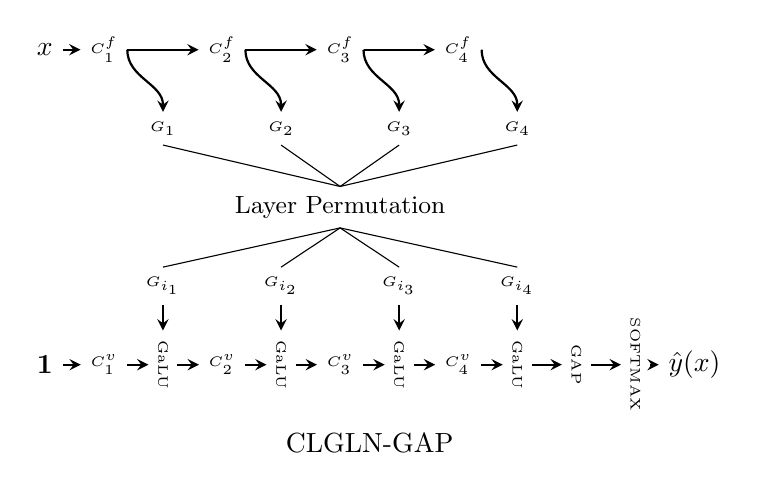
\begin{tikzpicture}
\node []  (fntext)at (-4.625,-3.5) {CLGLN-GAP};

%\node []  (output) at (7.5,1.5) {$\hat{y}(x)$};


\node [] (dgn1-f-c4) at (-3.5,1.5){\tiny{$C^{\text{f}}_4$}};
\node [] (dgn1-f-c3) at (-5,1.5){\tiny{$C^{\text{f}}_3$}};
\node [] (dgn1-f-c2) at (-6.5,1.5){\tiny{$C^{\text{f}}_2$}};
\node [] (dgn1-f-c1) at (-8,1.5){\tiny{$C^{\text{f}}_1$}};
\node [] (dgn1-input-f) at (-8.75,1.5){$x$};
\draw [-stealth,thick]   (dgn1-f-c3.east) -- (dgn1-f-c4.west);
\draw [-stealth,thick]   (dgn1-f-c2.east) -- (dgn1-f-c3.west);
\draw [-stealth,thick]   (dgn1-f-c1.east) -- (dgn1-f-c2.west);
\draw [-stealth,thick]   (dgn1-input-f.east) -- (dgn1-f-c1.west);



\node []  (dgn1-output) at (-0.5,-2.5) {$\hat{y}(x)$};

\node [rotate=-90] (dgn1-smax) at (-1.25,-2.5){\tiny{SOFTMAX}};
\draw [-stealth,thick]   (dgn1-smax.north)--(dgn1-output.west);

\node [rotate=-90] (dgn1-gap) at (-2,-2.5){\tiny{GAP}};
\draw [-stealth,thick]   (dgn1-gap.north)--(dgn1-smax.south);


\node [rotate=-90] (dgn1-galu-4) at (-2.75,-2.5){\tiny{GaLU}};
\draw [-stealth,thick]   (dgn1-galu-4.north)--(dgn1-gap.south);

\node [] (dgn1-v-c4) at (-3.5,-2.5){\tiny{$C^{\text{v}}_4$}};
\draw [-stealth,thick]   (dgn1-v-c4.east) -- (dgn1-galu-4.south);


\node [rotate=-90] (dgn1-galu-3) at (-4.25,-2.5){\tiny{GaLU}};
\draw [-stealth,thick]   (dgn1-galu-3.north) -- (dgn1-v-c4.west);

\node [] (dgn1-v-c3) at (-5,-2.5){\tiny{$C^{\text{v}}_3$}};
\draw [-stealth,thick]   (dgn1-v-c3.east) -- (dgn1-galu-3.south);


\node [rotate=-90] (dgn1-galu-2) at (-5.75,-2.5){\tiny{GaLU}};
\draw [-stealth,thick]   (dgn1-galu-2.north) -- (dgn1-v-c3.west);

\node [] (dgn1-v-c2) at (-6.5,-2.5){\tiny{$C^{\text{v}}_2$}};
\draw [-stealth,thick]   (dgn1-v-c2.east) -- (dgn1-galu-2.south);


\node [rotate=-90] (dgn1-galu-1) at (-7.25,-2.5){\tiny{GaLU}};
\draw [-stealth,thick]   (dgn1-galu-1.north) -- (dgn1-v-c2.west);


\node [] (dgn1-v-c1) at (-8,-2.5){\tiny{$C^{\text{v}}_1$}};
\draw [-stealth,thick]   (dgn1-v-c1.east) -- (dgn1-galu-1.south);


\node [] (dgn1-v-input) at (-8.75,-2.5){$\mathbf{1}$};

\draw [-stealth,thick]   (dgn1-v-input.east) -- (dgn1-v-c1.west);


\node[] (dgn1-gating-4-up) at (-2.75,0.5){\tiny{$G_{4}$}};
\draw [-stealth,thick]   (dgn1-f-c4.east) to[out=-90,in=90] (dgn1-gating-4-up.north);


\node[] (dgn1-gating-3-up) at (-4.25,0.5){\tiny{$G_{3}$}};
\draw [-stealth,thick]   (dgn1-f-c3.east) to[out=-90,in=90] (dgn1-gating-3-up.north);



\node[] (dgn1-gating-2-up) at (-5.75,0.5){\tiny{$G_{2}$}};
\draw [-stealth,thick]   (dgn1-f-c2.east) to[out=-90,in=90] (dgn1-gating-2-up.north);


\node[] (dgn1-gating-1-up) at (-7.25,0.5){\tiny{$G_{1}$}};
\draw [-stealth,thick]   (dgn1-f-c1.east) to[out=-90,in=90] (dgn1-gating-1-up.north);





\node[] (dgn1-gating-4) at (-2.75,-1.5){\tiny{$G_{i_4}$}};
\draw [-stealth,thick]   (dgn1-gating-4.south) -- (dgn1-galu-4.west);


\node[] (dgn1-gating-3) at (-4.25,-1.5){\tiny{$G_{i_3}$}};
\draw [-stealth,thick]   (dgn1-gating-3.south) -- (dgn1-galu-3.west);



\node[] (dgn1-gating-2) at (-5.75,-1.5){\tiny{$G_{i_2}$}};
\draw [-stealth,thick]   (dgn1-gating-2.south) -- (dgn1-galu-2.west);


\node[] (dgn1-gating-1) at (-7.25,-1.5){\tiny{$G_{i_1}$}};
\draw [-stealth,thick]   (dgn1-gating-1.south) -- (dgn1-galu-1.west);



\node[] (permutation1) at (-5,-0.5){\small{Layer Permutation}};

\draw [-]   (dgn1-gating-1-up.south) -- (permutation1.north);
\draw [-]   (dgn1-gating-4-up.south) -- (permutation1.north);
\draw [-]   (dgn1-gating-2-up.south) -- (permutation1.north);
\draw [-]   (dgn1-gating-3-up.south) -- (permutation1.north);



\draw [-]  (permutation1.south) --  (dgn1-gating-1.north)  ;
\draw [-]  (permutation1.south) --  (dgn1-gating-2.north)  ;
\draw [-]  (permutation1.south) --  (dgn1-gating-3.north)  ;
\draw [-]  (permutation1.south) --  (dgn1-gating-4.north)  ;


%%%%%%%%%%%%%%%%%%%%%%%%%%%%%%%%%%%%%%%%%%%%%%%%%%%%%%%%%%%%%%%%%

	
\end{tikzpicture}


}
\end{minipage}
\end{minipage}
\caption{$4$ convolutional layers with GAP}
\label{fig:c4gap}
\end{figure}
\end{comment}

\begin{table}[!t]
\centering
\resizebox{1.0\columnwidth}{!}{
\begin{tabular}{ccccccc}
\toprule 
Dataset 					& C4GAP 		&DNN 	&DGN$(x,x)$ 			&DGN$(x,\mathbf{1})$ 	&DLGN$(x,x)$ 			&DLGN$(x,\mathbf{1})$ 	\\\midrule
\multirow{2}{*}{CIFAR10}		& Vanilla				&80.5\tiny{$\pm$0.4} 	&77.4\tiny{$\pm$0.3} 	& 77.5\tiny{$\pm$0.2} 	&75.4\tiny{$\pm$0.3} 	&75.4\tiny{$\pm$0.2}		\\
						& Permute 	&-- 		&77.3\tiny{$\pm$0.5} 	&77.9\tiny{$\pm$0.6}		&75.9\tiny{$\pm$0.5} 	&76.0\tiny{$\pm$0.5}		\\%\midrule
%\multirow{2}{*}{CIFAR100}		& Vanilla  				&51.8\tiny{$\pm$0.4} 	&47.4\tiny{$\pm$0.2}		&47.3\tiny{$\pm$0.3} 	&47.4\tiny{$\pm$0.1} 	&48.0\tiny{$\pm$0.2}		\\
%						& Permute 	& -- 		&48.4\tiny{$\pm$0.8} 	&49.2\tiny{$\pm$0.9} 	&47.5\tiny{$\pm$1.0} 	&48.4\tiny{$\pm$0.9}		\\
\bottomrule
\end{tabular}
}
\caption{\tiny{Disentangling in path space.}}
\label{tb:permute}
\end{table}

\begin{table}[!t]
\centering
%\resizebox{1.0\columnwidth}{!}{
\begin{tabular}{ccccccccc}
\toprule 
Dataset 					& Model 		&DNN 				&DGN$(x,x)$ 			&DGN$(x,\mathbf{1})$ 	&DLGN$(x,x)$ 			&DLGN$(x,\mathbf{1})$ 	\\\midrule		
\multirow{2}{*}{CIFAR10}		&VGG16 		&93.6\tiny{$\pm$0.2} 	& 93.0\tiny{$\pm$0.1}  	&93.0\tiny{$\pm$0.1}   	&87.0\tiny{$\pm$0.1}		&87.0\tiny{$\pm$0.2}		\\
						&ResNet110 	&94.0\tiny{$\pm$0.2} 	& 93.3\tiny{$\pm$0.2} 	&93.2\tiny{$\pm$0.1} 	&87.9\tiny{$\pm$0.2}   	&87.8\tiny{$\pm$0.1} 	\\\midrule
\multirow{2}{*}{CIFAR100}		&VGG16	 	&73.4\tiny{$\pm$0.3}  	&70.3\tiny{$\pm$0.1} 	&70.5\tiny{$\pm$0.2} 	&61.5\tiny{$\pm$0.2}		&61.5\tiny{$\pm$0.1}		\\
						&ResNet110 	&72.7\tiny{$\pm$0.2}		&70.8\tiny{$\pm$0.2} 	&70.8\tiny{$\pm$0.4}		&62.3\tiny{$\pm$0.2} 	&62.7\tiny{$\pm$0.3} 	\\
\bottomrule
\end{tabular}
%}
\caption{Summary of Experiments}
\label{tb:expresults}
\end{table}


\begin{comment}
\begin{table}[!t]
\centering
\resizebox{1.0\columnwidth}{!}{
\begin{tabular}{ccccccccc}
\toprule 
Dataset 					& Model 				&DNN 				&DGN$(x,x)$ 			&DGN$(x,\mathbf{1})$ 	&DLGN$(x,x)$ 			&DLGN$(x,\mathbf{1})$ 	&DSLGN$(x,x)$ 		&DSLGN$(x,\mathbf{1})$  \\\midrule
\multirow{2}{*}{CIFAR10}		& C4GAP 				&80.5\tiny{$\pm$0.4} 	&77.4\tiny{$\pm$0.3} 	& 77.5\tiny{$\pm$0.2} 	&75.4\tiny{$\pm$0.3} 	&75.4\tiny{$\pm$0.2}		&74.2\tiny{$\pm$0.2}	 	&73.3\tiny{$\pm$0.2} \\
						& C4GAP-PERMUTE 	&-- 					&77.3\tiny{$\pm$0.5} 	&77.9\tiny{$\pm$0.6}		&75.9\tiny{$\pm$0.5} 	&76.0\tiny{$\pm$0.5}		& -- 					& -- \\\midrule
\multirow{2}{*}{CIFAR100}		& C4GAP 				&51.8\tiny{$\pm$0.4} 	&47.4\tiny{$\pm$0.2}		&47.3\tiny{$\pm$0.3} 	&47.4\tiny{$\pm$0.1} 	&48.0\tiny{$\pm$0.2}		&45.8\tiny{$\pm$0.3}	 	&44.9\tiny{$\pm$0.1}	\\
						& C4GAP-PERMUTE 	& -- 					&48.4\tiny{$\pm$0.8} 	&49.2\tiny{$\pm$0.9} 	&47.5\tiny{$\pm$1.0} 	&48.4\tiny{$\pm$0.9}		& --					& -- \\
\bottomrule
\end{tabular}
}
\caption{Summary of Experiments}
\label{tb:premresults}
\end{table}

\begin{table}[!t]
\centering
\resizebox{1.0\columnwidth}{!}{
\begin{tabular}{ccccccccc}
\toprule 
Dataset 					& Model 		&DNN 				&DGN$(x,x)$ 			&DGN$(x,\mathbf{1})$ 	&DLGN$(x,x)$ 			&DLGN$(x,\mathbf{1})$ 	&DSLGN$(x,x)$ 		&DSLGN$(x,\mathbf{1})$  \\\midrule		
\multirow{2}{*}{CIFAR10}		&VGG16-AP 	&93.6\tiny{$\pm$0.2} 	& 93.0\tiny{$\pm$0.1}  	&93.0\tiny{$\pm$0.1}   	&87.0\tiny{$\pm$0.1}		&87.0\tiny{$\pm$0.2}		&84.8\tiny{$\pm$0.3} 	&84.9\tiny{$\pm$0.2} \\
						&ResNet110 	&94.0\tiny{$\pm$0.2} 	& 93.3\tiny{$\pm$0.2} 	&93.2\tiny{$\pm$0.1} 	&87.9\tiny{$\pm$0.2}   	&87.8\tiny{$\pm$0.1} 	&72.4{$\pm$13.8} 		&71.2{$\pm$17.3}  \\\midrule
\multirow{2}{*}{CIFAR100}		&VGG16-AP 	&73.4\tiny{$\pm$0.3}  	&70.3\tiny{$\pm$0.1} 	&70.5\tiny{$\pm$0.2} 	&61.5\tiny{$\pm$0.2}		&61.5\tiny{$\pm$0.1}		&56.4\tiny{$\pm$0.4} 	&56.3\tiny{$\pm$0.2}\\
						&ResNet110 	&72.7\tiny{$\pm$0.2}		&70.8\tiny{$\pm$0.2} 	&70.8\tiny{$\pm$0.4}		&62.3\tiny{$\pm$0.2} 	&62.7\tiny{$\pm$0.3} 	&49.8{$\pm$0.9}		&41.5{$\pm$15.5}  \\
\bottomrule
\end{tabular}
}
\caption{Summary of Experiments}
\label{tb:expresults}
\end{table}
\end{comment}
%& C4GAP 		& 51.8 \tiny{$\pm$0.4} 	& DGN$(x,x)$ 	& DGN$(x,\mathbf{1})$ 	&  DLGN$(x,x)$ 	& DLGN$(x,\mathbf{1})$ & DSLGN$(x,x)$ 	& DSLGN$(x,\mathbf{1})$\\




%We now present additional theoretical and experimental insights on dual linearity that show that the once the gates are given the learning in the weights is best understood by a path-by-path view and the layer-by-layer view is not relevant.



%Given a DNN, there are two corresponding networks, the LGLN  in \Cref{sec:intro} and the DGN in \Cref{sec:prelim}. The LGLN can be obtained from the DGN by,

%(i) replacing all the ReLU activations in the feature network 

%The DGN performs only marginally poor compared to the DNN, and by successfully addressing the `black box'-ness issue in a DGN we will have both performance and interpretability. We now propose our novel \texttt{DGN-NO-ACT}  which disentangles the computations into (i) primal linear layer-by-layer computation, (ii) dual linear path-by-path computation and (iii) gating non-linearity which \emph{lifts} the computations from the primal to the dual. \texttt{DGN-NO-ACT} (right diagram in \Cref{fig:dgn}) is obtained by making a novel modification to the DGN (left diagram in \Cref{fig:dgn}) as follows:

%1. We replace the ReLUs in the feature network with \emph{identity} maps, i.e., $I(q) = q$. Thus, in the \texttt{DGN-NO-ACT}, the transformation from input to the pre-activations is entirely linear. We call this \textbf{primal linearity}. The disentanglement happens because the ReLU  is completely removed.  

%2. The value network of the DGN is linear in dual `path' variables. We call this \textbf{dual linearity} which stands for the fact that the value network computes path-by-path, and not layer-by-layer. As a result, presenting a $\mathbf{1}$ as input to the value network in \texttt{DGN-NO-ACT} does not degrade performance. The simplifications are : (i) $v_{\Tv}\in \R^{\text{total\,paths}}$ is a vector that does not depend on the input, and (ii) $\phi_{\Tf}(x)\in(0,1)^{\text{total\,paths}}$ is a  simple feature vector. In other words, the value network  learns the paths, and the feature network learns the activations of paths for each input.  While in each layer of the value network GaLUs and the linear operations are entangled, disentanglement happens in the path variables, and we do not have to worry about how learning happens layer-by-layer.

%3. The gates themselves serve the functionality of \emph{lifting} the computations from the primal to the dual, i.e., pre-activations trigger the gates which in turn activate the paths.

%\textbf{Significance.} The salient importance of the \texttt{DGN-NO-ACT} is that it clearly separates the layer-by-layer computations in the feature network and path-by-path computation in the value network. The importance of primal linearity is that we can now use standard linear algebra to `mathematically' interpret the linear transformations from the input to the pre-activations. Also, in the case of specific application domains such as `image classification', these transformations are `filter banks' which have been extensively studied with well known interpretations. The `mathematical' as well as domain specific interpretabilities obviate the need for `locally linear explanation using simpler models': the feature network is entirely linear and is itself simple. The importance of dual linearity is that it gives us a \emph{kernel} based `mathematical' interpretation in the \emph{infinite width regime}. 


%\textbf{DGN-NO-ACT(our model)}(see right diagram in \Cref{fig:dgn}). We replace the ReLUs in the feature network with \emph{identity} maps, i.e., $I(q) = q$. Thus, in the \texttt{DGN-NO-ACT}, the transformation from input to the pre-activations is entirely linear and is amenable to interpertation via standard spectral analysis using linear algebraic tools. The pre-activations trigger the gates, which then dictates the path activity. The value network is given only given $\mathbf{1}$ as input and hence $v_{\Tv}\in \R^{\text{total\,paths}}$ is a vector that does not depend on the input, and $\phi_{\Tf}(x)\in(0,1)^{\text{total\,paths}}$ is a very simple feature vector. % and the output $\hat{y}_{\text{DGN}}(x)=\ip{\phi_{\Tf}(x),v_{\Tv}}=\sum_{p}\phi_\Tf(x,p)v_\Tv(p)$ is equal to \emph{\textbf{the summation of `path value' weighted by the `path activations'}}. 
%Thus, the \texttt{DGN-NO-ACT} can be seen to disentangle the `primal linear' feature network which generates the gates, which in turn activate the paths in the value network which is the `dual linear'.

%\textbf{Remark.} Presenting the value network with $\mathbf{1}$ is very counter intutive, which will get justfied in theory as well as experiments in the next section. As a quick check, we the test accuracies of a DNN $4$ with convolutional layers and global-average-pooling (GAP), its corresponding DGN and \texttt{DGN-NO-ACT} on CIFAR-10 are {\bf{DNN: $80.4\%$,  DGN: $77.4\%$, \texttt{DGN-NO-ACT} : $74.5\%$}}.

%Since $\hat{y}_{\Theta}(x)=\ip{\phi_{x,\Theta},v_{\Theta}}$, during training, as $\Theta$ is learnt, both the NPFs and NPV are also learnt. To understand their roles better, $\phi_{x,\Theta}$ and $v_{\Theta}$ have to be separated.  This is achieved by the deep gated network (DGN) setup (see \Cref{fig:dgn}), which has two networks of \emph{identical architecture} namely the \emph{feature network} ($\Tf\in\R^{d^{\text{f}}_{\text{net}}}$) which holds the NPFs (i.e., the gating information) and the \emph{value network} ($\Tv\in\R^{d^{\text{v}}_{\text{net}}}$) which holds the NPV.  The combined parameterisation is denoted by $\Theta^{\text{DGN}}=(\Tf,\Tv)\in \R^{d^{\text{f}}_{\text{net}}+d^{\text{v}}_{\text{net}}}$.  The feature network is a DNN with ReLUs and the value network is a DNN with \emph{Gated Linear Units (GaLUs)} (terminology used in [\citenum{sss}]) whose output is the product of its pre-activation input $q^{\text{v}}(x)$and the external gating signal $G^{\text{f}}(x)$ (see \Cref{fig:dgn}). In \Cref{fig:dgn}, the main output of the DGN is $\hat{y}_{\text{DGN}}(x)$, while the other output $\hat{y}_{\text{f}}(x)$ is used to \emph{pre-train} the gates (see \Cref{sec:exp}).

